\documentclass{article}
%\usepackage{fullpage}
%\usepackage{nopageno} 
\usepackage[margin=1.5in]{geometry}
\usepackage{tikz}
\usetikzlibrary{shapes.geometric, calc}
\usepackage{amsmath}
\usepackage{amssymb}
\usepackage[normalem]{ulem}
\usepackage{fancyhdr}
\usepackage{cancel}
\usepackage{enumerate}
%\renewcommand\headheight{12pt}
\pagestyle{fancy}
\lhead{April 25, 2014}
\rhead{Jon Allen}
\allowdisplaybreaks

\newcommand{\abs}[1]{\left\lvert #1 \right\rvert}

\begin{document}
\section*{Chapter 7}
\begin{enumerate}
  \setcounter{enumi}{32}
  \item
  Solve the recurrence relation $h_n=h_{n-1}+9h_{n-2}-9h_{n-3},\quad(n\ge3)$ with initial values $h_0=0,h_1=1,$ and $h_2=2$.
  \begin{align*}
    0&=h_n-h_{n-1}-9h_{n-2}+9h_{n-3}\\
    0&=q^3-q^2-9q+9\\
    0&=(q+a)(q^2+bq+c)=q^3+(b+a)q^2+(ab+c)q+ac\\
    &=(q-3)(q^2+bq-3)=q^3+(b-3)q^2+(-3b-3)q+9\\
    &=(q-3)(q^2+2q-3)=(q-3)(q-1)(q+3)\\
    h_n&=c_1(3)^n+c_2(1)^n+c_3(-3)^n\\
    h_0=0&=c_1+c_2+c_3\\
    h_1=1&=3c_1+c_2-3c_3=3c_1+c_2+3c_1+3c_2=6c_1+4c_2\\
    h_2=2&=9c_1+c_2+9c_3=9c_1+c_2-9c_1-9c_2=-8c_2\\
    c_2&=-\frac{1}{4},\quad c_1=\frac{1}{3},\quad c_3=-\frac{1}{12}\\
    h_n&=\frac{4\cdot3^n-3-(-3)^n}{12}
  \end{align*}
  \item
  Solve the recurrence relation $h_n=8h_{n-1}-16h_{n-2},\quad(n\ge2)$ with initial values $h_0=-1$ and $h_1=0$.
  \begin{align*}
    0&=h_n-8h_{n-1}+16h_{n-2}\\
    0&=q^2-8q+16\\
    0&=(q-4)^2\\
    h_n&=c_14^n+c_2n4^n\\
    h_0={-1}&=c_1\\
    h_1=0&=-4+c_24,\quad c_2=1\\
    h_n&=-4^n+n4^n
  \end{align*}
  \setcounter{enumi}{36}
%  \item
%  (bonus)
%
%%  Determine a recurrence relation for the number $a_n$ of ternary strings (made up of 0s, 1s, and 2s) of length $n$ that do not contain two consecutive 0's or two consecutive 1s. Then find a formula for $a_n$
%
%\[a_n=2a_{n-1}+a_{n-2}\]
%
%  \[
%    \begin{matrix}
%    a_0=1&\emptyset\\
%    a_1=3&0&1&2\\
%    a_2=7&01&02&10&12&20&21&22\\
%    a_3=17&010&012&020&021&022&101&102&120&121\\
%      &122&201&202&210&212&220&221&222\\
%    a_4=41&0101&0102&0120&0121&0122&0201&0202&0210&0212\\
%      &0220&0221&0222&1010&1012&1020&1021&1022&1201\\
%      &1202&1210&1212&1220&1221&1222&2010&2012&2020\\
%      &2021&2022&2101&2102&2120&2121&2122&2201&2202\\
%      &2210&2212&2220&2221&2222
%    \end{matrix}
%  \]
  \setcounter{enumi}{37}
  \item
  Solve the following recurrence relations by examining the first few values for a formula andd then proving your conjectured formula by induction.
  \begin{enumerate}
    \setcounter{enumii}{1}
    \item
    $h_n=h_{n-1}-n+3,\quad(n\ge1);\;h_0=2$
    \begin{align*}
      h_0&=2&h_1&=2-1+3=4&h_2&=4-2+3=5&h_3&=5-3+3=5\\
      h_4&=5-4+3=4&h_5&=4-5+3=2&h_6&=2-6+3={-1}&h_7&=-1-7+3=-5
    \end{align*}
    I have no intuition whatsoever.
    \begin{align*}
      0&=h_n-h_{n-1}\\
      0&=q-1,\quad q=1\\
      h_n&=c\\
      \intertext{$rn+s$ give the impossible condition $r=r-1$}
      rn^2+sn+t&=r(n-1)^2+s(n-1)+t-n+3=r(n^2-2n+1)+sn-s+t-n+3\\
      &=rn^2-2rn+sn-n+r-s+t+3=rn^2+(-2r+s-1)n+r-s+t+3\\
      s&=-2r+s-1,\quad r=-\frac{1}{2}\\
      t&=r-s+t+3=-\frac{1}{2}-s+3+t,\quad s=\frac{5}{2}\\
      t&=0\\
      h_n&=c-\frac{1}{2}n^2+\frac{5}{2}n\\
      2&=c\\
      h_n&=2-\frac{1}{2}n^2+\frac{5}{2}n
    \end{align*}
    We don't exactly have a conjectured formula, but we will prove it anyhow. First by showing that $h_0=2$ and then by showing that $h_{n+1}=h_n-(n+1)+3$ which is the same as $h_n=h_{n-1}-n+3$
    \begin{align*}
      h_0&=2-\frac{1}{2}0^2+\frac{5}{2}0=2\\
      h_{n+1}&=2-\frac{1}{2}(n+1)^2+\frac{5}{2}(n+1)\\
      &=2-\frac{1}{2}n^2-n-\frac{1}{2}+\frac{5}{2}n+\frac{5}{2}\\
      &=2-\frac{1}{2}n^2+\frac{5}{2}n-n+2\\
      &=2-\frac{1}{2}n^2+\frac{5}{2}n-(n+1)+3\\
      h_n&=2-\frac{1}{2}n^2+\frac{5}{2}n\\
      h_{n+1}&=h_n-(n+1)+3
    \end{align*}
    And scene. $\Box$
  \end{enumerate}
  \setcounter{enumi}{39}
  \item
  Let $a_n$ equal the number of ternary strings of length $n$ made up of 0s, 1s, and 2s, such that the substrings 00, 01, 10, and 11 never occur. Prove that
\[a_n=a_{n-1}+2a_{n-2},\quad(n\ge2),\]
  with $a_0=1$ and $a_1=3$. Then find a formula for $a_n$.
\subsubsection*{proof}
  So let us take a sequence of length $n$.
  There are $a_n$ possibilities for the entire sequence, but only three possibilities for the last digit of the sequence.
  This number is the sum of the possible sequences that end in each possible digit.
  We will label the number of these possibilities with $_0a_{n-1}, _1a_{n-1},$ and $_2a_{n-1}$.
  Now if the $n$th digit in our sequence is 0 then we only have one choice (two) in the digit for $n-1$ and so ${_0a_{n-1}}=a_{n-2}$.
  Similarly ${_1a_{n-1}}=a_{n-2}$.
  Now if our $n$th digit is 2, then the possibilities for the previous digit are wide open, which  is to say ${_2a_{n-1}}=a_{n-1}$.
  Now putting it all together we see that $a_n={_0a_{n-1}}+{_1a_{n-1}}+{_2a_{n-1}}=a_{n-2}+a_{n-2}+a_{n-1}=a_{n-1}+2a_{n-2}$.
  And we have our result.
  $\Box$
  \subsubsection*{formula}
  \begin{align*}
    a_n&=a_{n-1}+2a_{n-2}\\
    0&=a_n-a_{n-1}-2a_{n-2}\\
    0&=q^2-q-2\\
    0&=(q+1)(q-2)\\
    a_n&=c_1({-1})^n+c_22^n\\
    a_0&=1=c_1+c_2\\
    a_1&=3=-c_1+2c_2\\
    c_1&=1-c_2\\
    3&=-(1-c_2)+2c_2=3c_2-1\\
    c_2&=\frac{4}{3},\quad c_1=-\frac{1}{3}\\
    a_n&=-\frac{1}{3}\cdot(-1)^n+\frac{4}{3}\cdot2^n
  \end{align*}
%  \item
%  (grad)
%
%  * Let $2n$ equally spaced points be chosen on a circle. Let $h_n$ denote the number of ways to join these points in pairs so that the resulting line segments do not intersect. Establish a recurrence relation for $h_n$.
  \setcounter{enumi}{43}
  \item
  Solve the nonhomogeneous recurrence relation
  \begin{align*}
    h_n&=3h_{n-1}-2,\quad(n\ge1)\\
    h_0&=1.
  \end{align*}
  First find homogeneous solutions
  \begin{align*}
    h_n&=3h_{n-1}\\
    0&=h_n-3h_{n-1}\\
    0&=q-3\\
    h_n&=c3^n\\
    h_n&=rn+s\\
    rn+s&=3(r(n-1)+s)-2\\
    &=3rn-3r+3s-2\\
    r&=3r=0\\
    s&=-3r+3s-2\\
    2s&=3r+2\\
    1&=3rn+\frac{1}{2}(3r+2)\\
    s&=\frac{1}{2}(3r+2)=1\\
    h_n&=1\to h_n=c3^n+1\\
    1&=c3^0+1\\
    0&=c\\
    h_n&=1
  \end{align*}
  \item
  Solve the nonhomogeneous recurrence relation
  \begin{align*}
    h_n&=2h_{n-1}+n,\quad(n\ge1)\\
    h_0&=1.
  \end{align*}
  \begin{align*}
    h_n&=2h_{n-1}\\
    0&=h_n-2h_{n-1}=q-2\\
    h_n&=c2^n\\
    rn+s&=2(r(n-1)+s)+n=2rn-2r+2s+n=(2r+1)n-2r+2s\\
    r&=2r+1\to r=-1\\
    s&=-2r+2s=2+2s\to s=-2\\
    h_n&=-n-2\\
    h_n&=c2^n-n-2\\
    1&=c-0-2\to c=3\\
    h_n&=3\cdot2^n-n-2
  \end{align*}
\end{enumerate}
\section*{Chapter 8}
Do two of 1,2 or 36
\begin{enumerate}
  \item
  Let $2n$ (equally spaced) points on a circle be chosen. Show that the number of ways to join these points in pairs, so that the resulting $n$ line segments do not intersect, equals the $n$th Catalan number $C_n$.
  \item
  Prove that the number of 2-by-$n$ arrays
  \[\begin{bmatrix}
    x_{11}&x_{12}&\dots&x_{1n}\\
    x_{21}&x_{22}&\dots&x_{2n}\\
  \end{bmatrix}\]
  that can be made from the numbers $1,2,\dots,2n$ such that
  \begin{align*}
    x_{11}<x_{12}<\dots<x_{1n},\\
    x_{21}<x_{22}<\dots<x_{2n}\\
  \end{align*}
  \[x_{11}<x_{21},x_{12}<x_{22},\dots,x_{1n}<x_{2n},\]
  equalsthe $n$th Catalan number, $C_n$.
  \item
  Write out all of the multiplication schemes for four numbers and the triangularization of a convex polygonal region of five sides corresponding to them.

  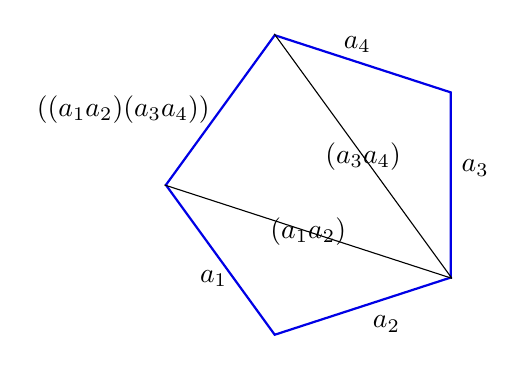
\begin{tikzpicture}

    \node (pol) [draw, thick, blue!90!black,rotate=90,minimum size=4cm,regular polygon, regular polygon sides=5] at (0,0) {}; 

    \foreach \n [count=\nu from 1, remember=\n as \lastn, evaluate={\nu+\lastn}] in {1,2,...,4} 
    \node[anchor=\n*(360/5)]at(pol.side \n){$a_{\nu}$};
    \draw (pol.corner 1) -- node{$(a_1 a_2)$}(pol.corner 3);
    \draw (pol.corner 3) -- node{$(a_3 a_4)$}(pol.corner 5);
    \node[anchor=5*(360/5)]at(pol.side 5){$((a_1 a_2)(a_3 a_4))$};

  \end{tikzpicture}
  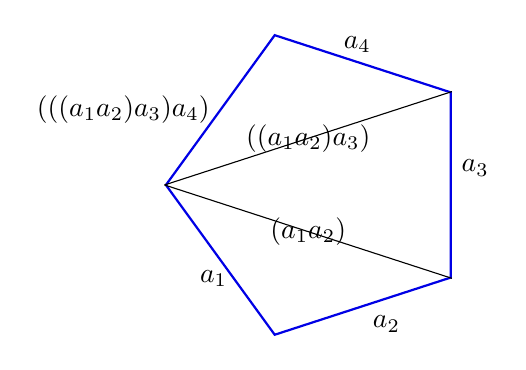
\begin{tikzpicture}

    \node (pol) [draw, thick, blue!90!black,rotate=90,minimum size=4cm,regular polygon, regular polygon sides=5] at (0,0) {}; 

    \foreach \n [count=\nu from 1, remember=\n as \lastn, evaluate={\nu+\lastn}] in {1,2,...,4} 
    \node[anchor=\n*(360/5)]at(pol.side \n){$a_{\nu}$};
    \draw (pol.corner 1) -- node{$(a_1 a_2)$}(pol.corner 3);
    \draw (pol.corner 1) -- node{$((a_1 a_2) a_3)$}(pol.corner 4);
    \node[anchor=5*(360/5)]at(pol.side 5){$(((a_1 a_2) a_3) a_4)$};

\end{tikzpicture}

  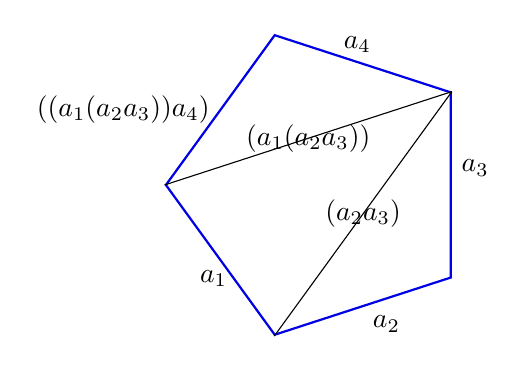
\begin{tikzpicture}

    \node (pol) [draw, thick, blue!90!black,rotate=90,minimum size=4cm,regular polygon, regular polygon sides=5] at (0,0) {}; 

    \foreach \n [count=\nu from 1, remember=\n as \lastn, evaluate={\nu+\lastn}] in {1,2,...,4} 
    \node[anchor=\n*(360/5)]at(pol.side \n){$a_{\nu}$};
    \draw (pol.corner 2) -- node{$(a_2 a_3)$}(pol.corner 4);
    \draw (pol.corner 1) -- node{$(a_1( a_2 a_3))$}(pol.corner 4);
    \node[anchor=5*(360/5)]at(pol.side 5){$((a_1( a_2 a_3))a_4)$};

\end{tikzpicture}
  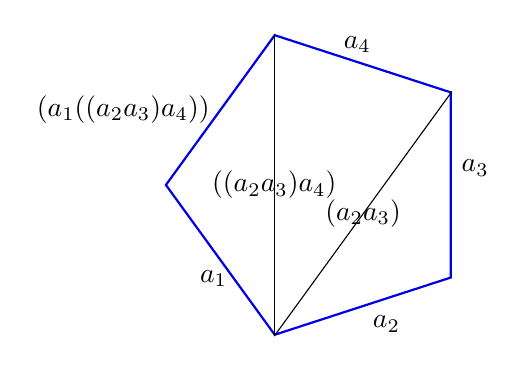
\begin{tikzpicture}

    \node (pol) [draw, thick, blue!90!black,rotate=90,minimum size=4cm,regular polygon, regular polygon sides=5] at (0,0) {}; 

    \foreach \n [count=\nu from 1, remember=\n as \lastn, evaluate={\nu+\lastn}] in {1,2,...,4} 
    \node[anchor=\n*(360/5)]at(pol.side \n){$a_{\nu}$};
    \draw (pol.corner 2) -- node{$(a_2 a_3)$}(pol.corner 4);
    \draw (pol.corner 2) -- node{$((a_2 a_3)a_4)$}(pol.corner 5);
    \node[anchor=5*(360/5)]at(pol.side 5){$(a_1((a_2 a_3)a_4))$};

\end{tikzpicture}

  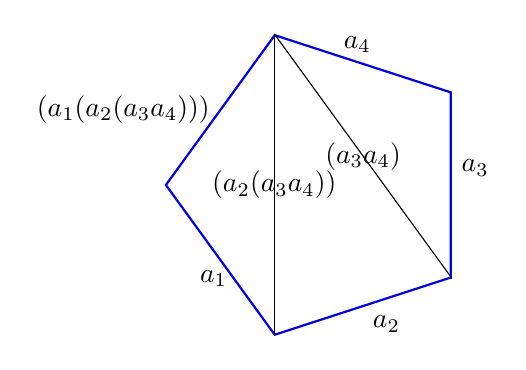
\begin{tikzpicture}

    \node (pol) [draw, thick, blue!90!black,rotate=90,minimum size=4cm,regular polygon, regular polygon sides=5] at (0,0) {}; 

    \foreach \n [count=\nu from 1, remember=\n as \lastn, evaluate={\nu+\lastn}] in {1,2,...,4} 
    \node[anchor=\n*(360/5)]at(pol.side \n){$a_{\nu}$};
    \draw (pol.corner 3) -- node{$(a_3a_4)$}(pol.corner 5);
    \draw (pol.corner 2) -- node{$(a_2(a_3a_4))$}(pol.corner 5);
    \node[anchor=5*(360/5)]at(pol.side 5){$(a_1(a_2(a_3a_4)))$};

\end{tikzpicture}
  \item
  Determine the triangularization of a convex polygonal region corresponding to the following multiplication schemes:
  \begin{enumerate}
    \item
    $(a_1\times(((a_2\times a_3)\times(a_4\times a_5))\times a_6))$

  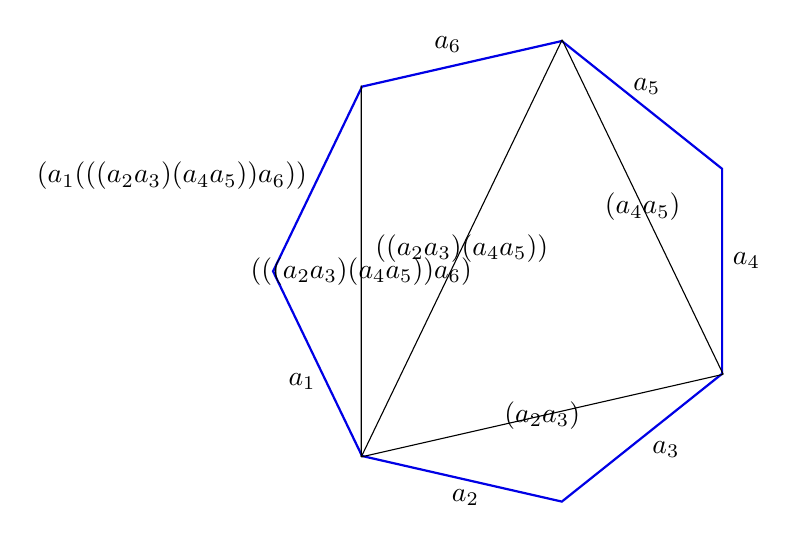
\begin{tikzpicture}

    \node (pol) [draw, thick, blue!90!black,rotate=90,minimum size=6cm,regular polygon, regular polygon sides=7] at (0,0) {}; 

    \foreach \n [count=\nu from 1, remember=\n as \lastn, evaluate={\nu+\lastn}] in {1,2,...,6} 
    \node[anchor=\n*(360/7)]at(pol.side \n){$a_{\nu}$};
    \draw (pol.corner 2) -- node{$(a_2 a_3)$}(pol.corner 4);
    \draw (pol.corner 4) -- node{$(a_4 a_5)$}(pol.corner 6);
    \draw (pol.corner 2) -- node{$((a_2 a_3)(a_4 a_5))$}(pol.corner 6);
    \draw (pol.corner 2) -- node{$(((a_2 a_3)(a_4 a_5)) a_6)$}(pol.corner 7);
    \node[anchor=7*(360/7)]at(pol.side 7){$(a_1(((a_2 a_3)(a_4 a_5)) a_6))$};

\end{tikzpicture}
    \item
    $(((a_1\times a_2)\times(a_3\times(a_4\times a_5)))\times((a_6\times a_7)\times a_8))$

  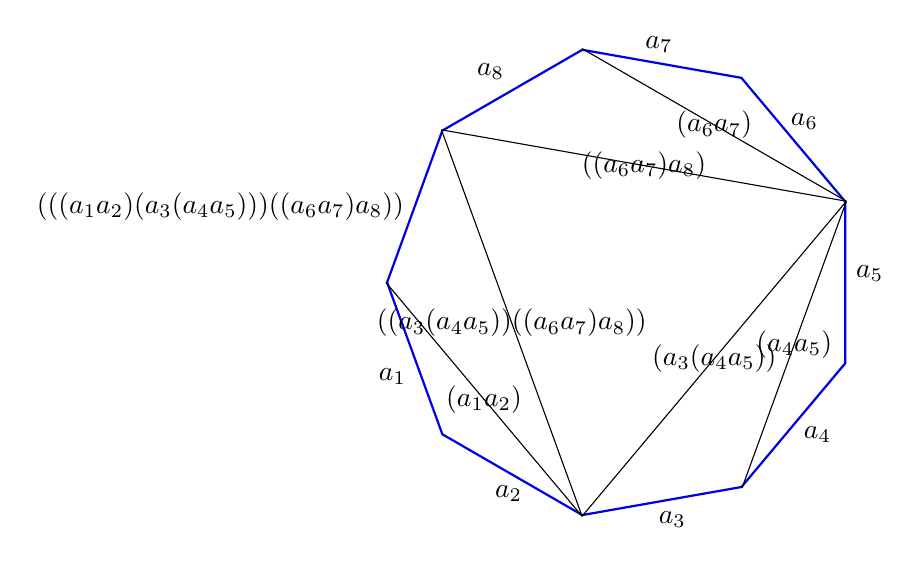
\begin{tikzpicture}

    \node (pol) [draw, thick, blue!90!black,rotate=90,minimum size=6cm,regular polygon, regular polygon sides=9] at (0,0) {}; 

    \foreach \n [count=\nu from 1, remember=\n as \lastn, evaluate={\nu+\lastn}] in {1,2,...,8} 
    \node[anchor=\n*(360/9)]at(pol.side \n){$a_{\nu}$};
    \draw (pol.corner 1) -- node{$(a_1 a_2)$}(pol.corner 3);
    \draw (pol.corner 4) -- node{$(a_4 a_5)$}(pol.corner 6);
    \draw (pol.corner 3) -- node{$(a_3(a_4 a_5))$}(pol.corner 6);
    \draw (pol.corner 6) -- node{$(a_6 a_7)$}(pol.corner 8);
    \draw (pol.corner 6) -- node{$((a_6 a_7) a_8)$}(pol.corner 9);
    \draw (pol.corner 3) -- node{$((a_3(a_4 a_5))((a_6 a_7) a_8))$}(pol.corner 9);
    \node[anchor=360]at(pol.side 9){$(((a_1 a_2)(a_3(a_4 a_5)))((a_6 a_7) a_8))$};

\end{tikzpicture}
  \end{enumerate}
  \setcounter{enumi}{35}
  \item
  Prove that the Catalan number $C_n$ equals the number of lattice paths from ${(0,0)}$ to ${(2n,0)}$ using only upsteps ${(1,1)}$ and downsteps ${(1,{-1})}$ that never go above the horizontal axis (so there are as many upsteps as there are downsteps). (These are sometimes call \emph{Dyck paths}.)
\subsubsection*{proof}
The number $a_{2n}$ of paths from (0,0) to $(0,2n)$ is the number of sequences of upsteps $(1,1)$ and downsteps $(1,-1)$ where the sum of the second coordinates is always negative. Because the first coordinate is always 1 this is the same as a sequence of n ones and n -1's whose partial sums are always negative. We can multiply each element in each sequence by -1. This gives us the smae number of sequences, however the partial sums of these sequences is always positive. Now we see from Theorem 8.1.1 that the number of these sequences is the nth Catalan number. $\Box$
\end{enumerate}
\end{document}
